\chapter{案例分析}
\section{案例實驗設計}\label{s4.1}
\indent
本論文以免費模板網頁Free CSS中的其中一個模板當基礎,
在原有的設計下做小幅度的修改,以此來作為此實驗的實驗網頁。
我們挑選出五個在撰寫測試腳本時時常會遇到的情況,
將情況設計成實驗案例來讓實驗人員實際操作。

在實驗人員的挑選中,
我們找了有網頁測試相關經驗的和對此技術較為陌生兩種類別的人,
最後會進行操作時間的比較。
為因應目前疫情時間,測試環境為同一台電腦以及硬體配備,
若為實體操作的話現場操作電腦,
若為遠端操作的話則使用Window遠端連線到該電腦來進行操作,
為確保實體和遠端的操作環境相同,遠端設備皆有檢測網速在50Mbps以上,並不會有遲鈍的現象。
操作的鍵盤滑鼠均屬於自己平時在使用的設備,
使用的介面為Chrome瀏覽器,工具為Chrome劉覽器中的Developer Tools和本實驗提出的擴充元件。

實驗流程開始前,
會先對測試人員用同一個簡報簡易說明該論文的背景知識、測試目的以及實驗網頁的簡單介紹,
之後會操作一個簡易的範例給實驗人員觀摩並且給實驗人員親自操作來熟悉該工具,
等一切初始程序就位後才會開始操作實驗案例,並記錄操作時間。

\section{測試案例實作}\label{s4.2}
挑選模板中,以互動功能多的網站為第一優先條件。
在眾多模板多,使用以家具為主的網頁模板\cite{Furn-Free-CSS-Template}來做實驗對象。

\begin{figure}[H]
    \centering
    \includegraphics[width=0.9\textwidth]{picture/experiment/test-environment-demo.png}
    \caption{實驗模板網站}
    \label{f4.1}
\end{figure}

\indent

\subsection{案例一:Hover購物車圖示後出現購物車下拉式畫面}\label{s4.2.1}
\indent
實驗者的測試情境為將滑鼠放在購物車的圖示上,
等到下拉式畫面出現後,需要找出所有因為下拉式畫面而屬性出現變化的元件,,如圖\ref{f4.2}所示。

該案例共有兩個元件有屬性變化,如果測試者皆找出變化並指出在Dev Tools中的位置則計為成功並記錄秒數。

\begin{figure}[H]
    \centering
    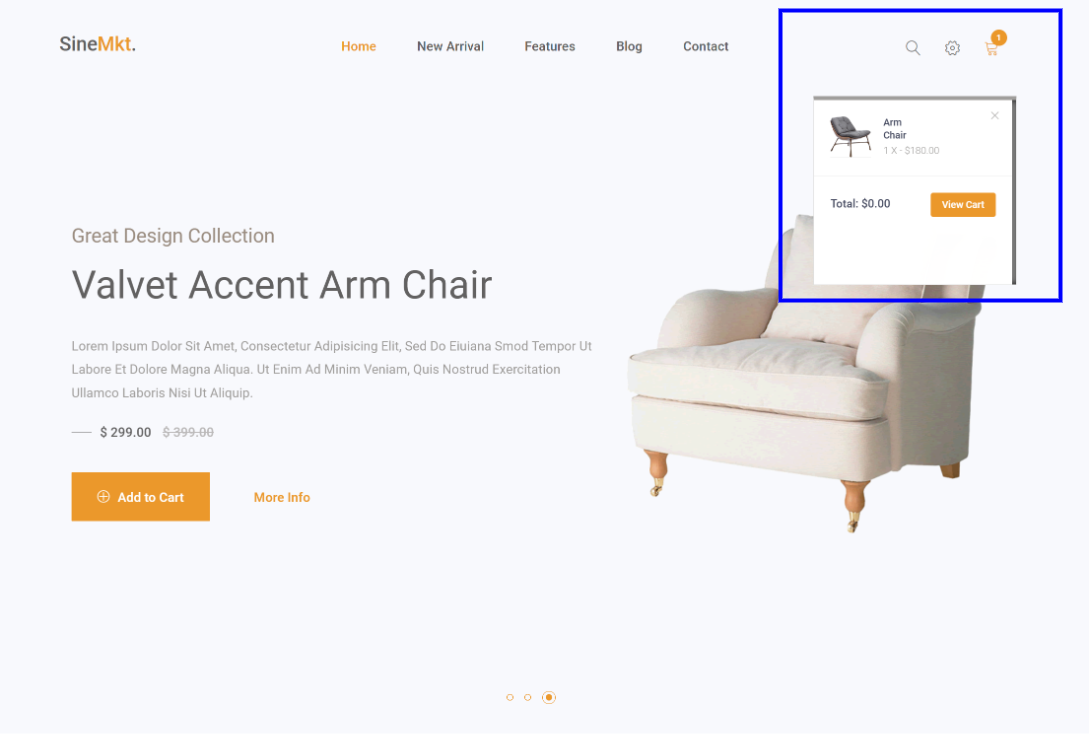
\includegraphics[width=0.6\textwidth]{picture/experiment/test-environment-no1.png}
    \caption{Hover購物車圖示後出現下拉示畫面之網頁變化}
    \label{f4.2}
\end{figure}

\subsection{案例二:點擊搜尋框後,僅需要了解該元件屬性變化}\label{s4.2.2}
\indent
實驗者的測試情境為利用點擊搜尋圖標後,可以將隱藏的搜尋框展開,
並找出有因為此互動而有變化的元件,如圖\ref{f4.3}所示。

該案例需要找出一個指定元件的屬性變化,如果測試者皆找出變化並指出在Dev Tools中的位置則計為成功並記錄秒數。

在此情境中,使用者可以使用擴充元件中"Only display change of current selecting elemnt"的Option,
讓測試者可以利用該Option過濾掉其餘畫面中不是搜尋框的變化並指出在Dev Tools中的位置,讓使用者專注在指定元件的屬性中。

\begin{figure}[H]
    \centering
    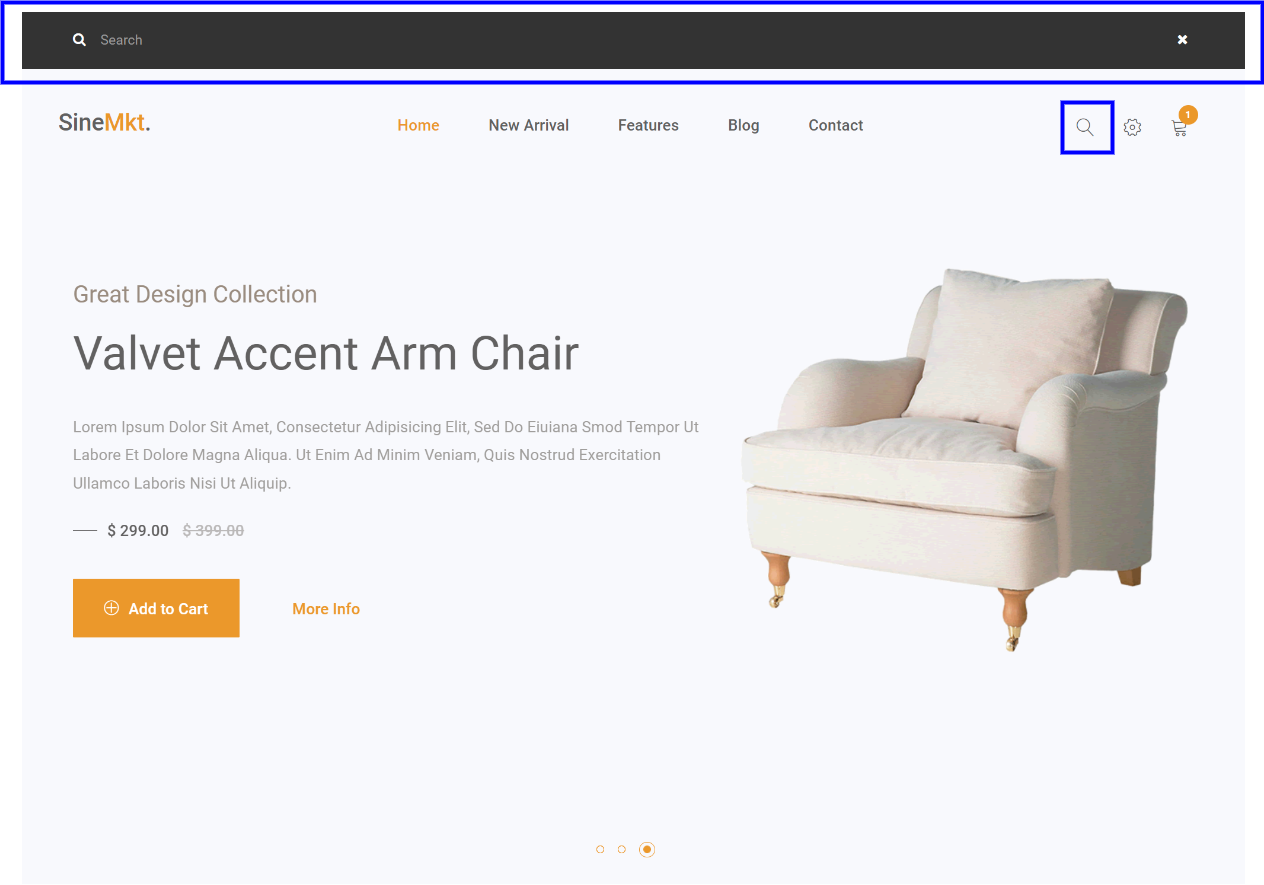
\includegraphics[width=0.6\textwidth]{picture/experiment/test-environment-no2.png}
    \caption{點擊搜尋圖包後之網頁變化}
    \label{f4.3}
\end{figure}

\subsection{案例三:網頁中畫面定時更換內容}\label{s4.2.3}
\indent
實驗者的測試情境為在網頁中的產品促銷頁面定時會更換的情況下,找出因為畫面更換而屬性出現變化的元件。
在此產品促銷頁面中,有三個子頁面,裡面各有一個促銷商品。
若使用者的滑鼠鼠標沒有在促銷頁面上,
它會定時滑動並道不同的內容中,
讓使用者即使不用操作頁面也可以看到每個在頁面上的促銷商品,如圖\ref{f4.4}所示。

該案例需要找出四個元件的屬性變化,如果測試者皆找出變化並指出在Dev Tools中的位置則計為成功並記錄秒數。

\begin{figure}[H]
    \centering
    \includegraphics[width=0.7\textwidth]{picture/experiment/test-environment-no3.png}
    \caption{產品促銷頁面循環示意圖}
    \label{f4.4}
\end{figure}


\subsection{案例四:點擊上方導覽列跳轉到該類別畫面}\label{s4.2.4}
\indent
實驗者的測試情境為點擊網頁上方的導覽列,可以快速跳轉到該網頁的指定區塊,讓使用者不用花費多餘的時間尋找該區塊在頁面中的位置,如圖\ref{f4.5}所示。

一般在畫面快速跳轉的情況下,無法快速地知道那些元件屬性有改變到,且必須要從整個網頁中慢慢尋找,會花相對多的時間在找差異,
透過此工具,可以快速地找到差異,並給測試者查看是否適合當Xpath表達式的條件。

該案例需要找出四個元件的屬性變化,如果測試者皆找出變化並指出在Dev Tools中的位置則計為成功並記錄秒數。

\begin{figure}[H]
    \centering
    \includegraphics[width=0.5\textwidth]{picture/experiment/test-environment-no4.png}
    \caption{利用導覽列跳轉到其他畫面之示意圖}
    \label{f4.5}
\end{figure}

\indent

\subsection{案例五:互動後當下網頁畫面無變化}\label{s4.2.5}
\indent
實驗者的使用情境為點擊促銷頁面中的按鈕後,
在當下畫面中因為變化中的元件沒有在畫面中,所以使用者在當下無法看不出有任何變化,也無法確保沒有任何元件被此點擊的動作影響到屬性。
如圖\ref{f4.5}所示,點擊按鈕後下方的標題會新增一行額外的文字,因為當下畫面是沒有變化的,所以使用者較難找出差別。

該案例需要找出一個被添加的元件,如果測試者找出變化並指出在Dev Tools中的位置則計為成功並記錄秒數。

\begin{figure}[H]
    \centering
    \includegraphics[width=0.5\textwidth]{picture/experiment/test-environment-no5.png}
    \caption{當下網頁中無包括有變化的元件之示意圖}
    \label{f4.6}
\end{figure}

\section{實驗數據分析}\label{s4.3}
\indent
本次實驗共有14位實驗人員參與,分成無相關經驗的7位以及有相關經驗的7位,藉由實驗人員的操作時間來比較有無使用此工具之差別。

由圖\ref{f4.7}可看出在實驗人員皆無相關經驗的情況下,
若使用操作工具在五個實例的情況中,減少的時間皆有25\%以上,甚至實例五有高達70\%左右。
% 減少時間:
%實例一: 0.738
%實例二: 0.516
%實例三: 0.621
%實例四: 0.675
%實例五: 0.279

\begin{figure}[H]
    \centering
    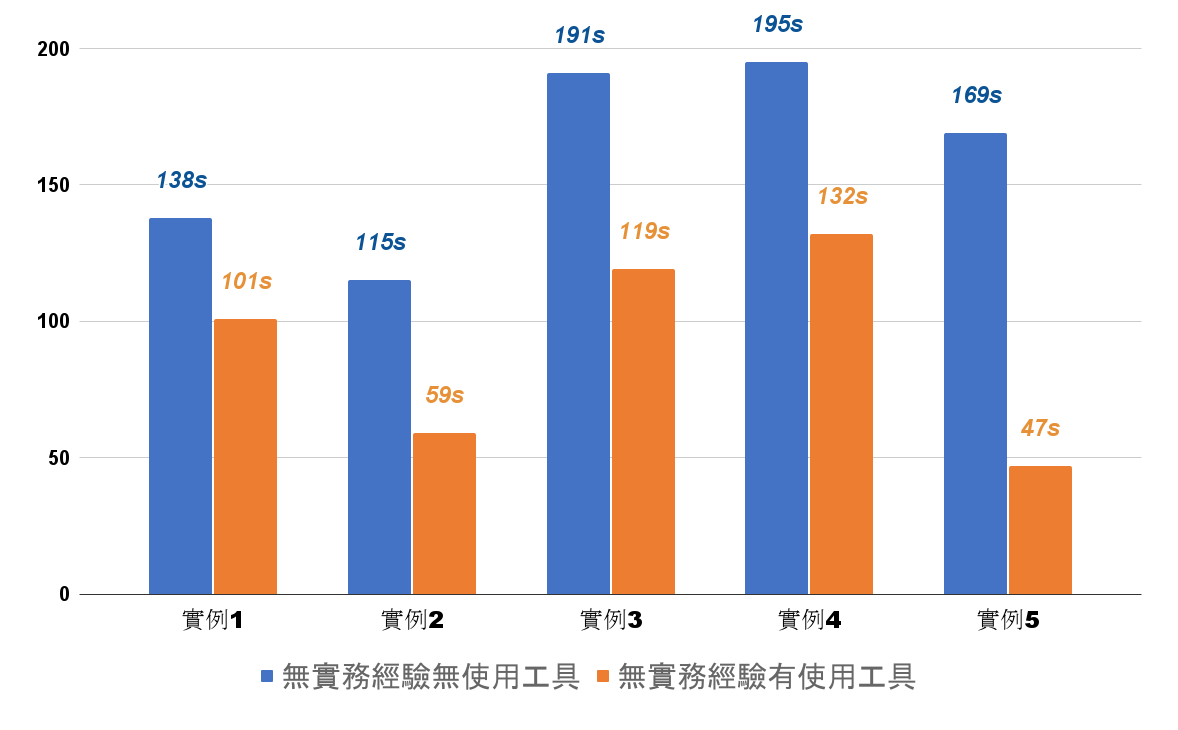
\includegraphics[width=0.8\textwidth]{picture/experiment/ch4-no_experience_compare.png}
    \caption{無實務經驗實驗人員操作時間比較}
    \label{f4.7}
\end{figure}

由圖\ref{f4.8}可看出在實驗人員有相關經驗的情況下,
實例二雖然時間很相近,
但實例二的實作過程因為只要找尋一個元件的變化,有相關經驗的人平時在找尋條件時也都只會看當下的元件,所以實驗結果是可以預期的。
其餘四個實例若使用操作工具減少的時間也有在20\%左右。

% 減少時間:
%實例一: 0.843
%實例二: 0.934
%實例三: 0.7084
%實例四: 0.6943
%實例五: 0.17788

\begin{figure}[H]
    \centering
    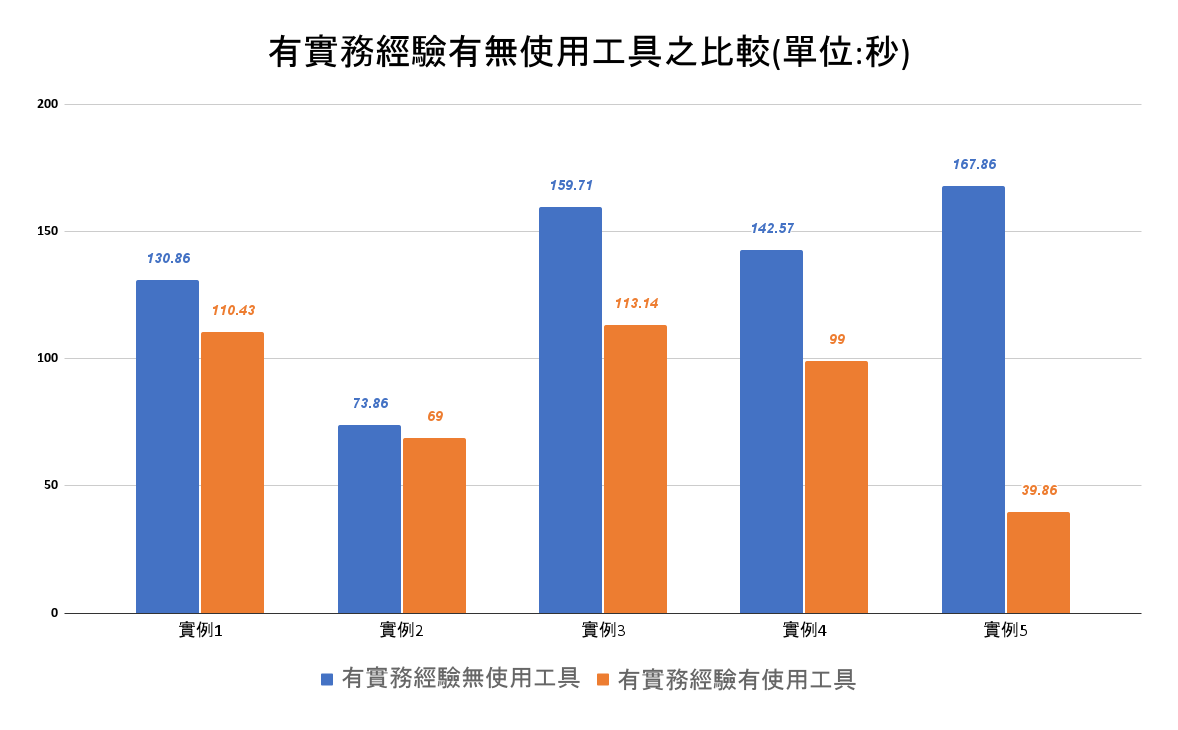
\includegraphics[width=0.8\textwidth]{picture/experiment/ch4-have_experience_compare.png}
    \caption{有實務經驗實驗人員操作時間比較}
    \label{f4.8}
\end{figure}

由圖\ref{f4.9}的全部實驗人員的時間統計下,可以看出每個實例都有減少20\%~30\%左右的時間,
其中案例五在有經驗或無經驗的情況下,時間皆大幅減少,由此可以看出即使有經驗的實驗人員,也較難找出超出畫面外的元件變化。

\begin{figure}[H]
    \centering
    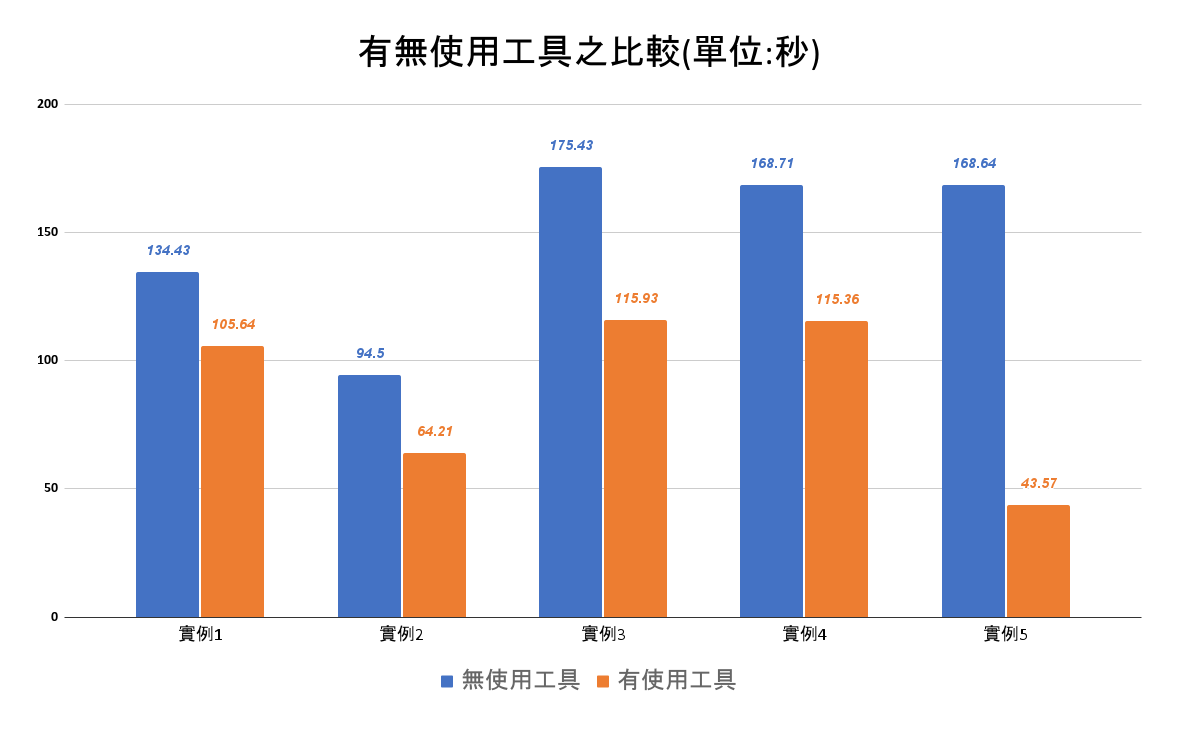
\includegraphics[width=0.8\textwidth]{picture/experiment/ch4-all_compare.png}
    \caption{全部實驗人員操作時間比較}
    \label{f4.9}
\end{figure}



% 設備:   電腦+遠端(因應疫情關係)
%         電腦採遠端,鍵盤滑鼠均採用自己習慣的    

% 測試人員:預計人數14人
% (有關專案*7)
% (X)-> 華暄Josie 
% (O)-> 彥文(OK)
% (X)-> 方子元
% (O)-> 陳志賢Larry)(OK)
% (X)-> 大四專題生*3

% (無關專案*7)(暫定)
% (-)-> 大三專題生*2
% (-)-> 碩零*2 (子龍 + 博士生)
% (X)-> 新允
% (O)-> 伯全(完成)
% (O)-> 承岳

% 設計情境 *  (本實驗僅只需要找出文本差異即可,不需要讓實驗者設計一個xpath表達式)

% 1.

% 測試目的:使用Navbar hover後文本出現的變化 (for timer功能)

% 使用前+使用後時間:

% 2.

% 測試目的:點擊按鈕後,部分網頁出現之變化 (for add remove)

% 使用前+使用後時間:

% 3.

% 測試目的: 點擊按鈕後,某個元件屬性出現變化(for change type)

% 使用前+使用後時間:

% 4.

% 測試目的: 網頁往下移動,但元件沒有任何變化(for no change)

% 使用前+使用後時間:

% 5.

% 測試目的: 點擊後有兩個元件會變化(一個只有style會變化,一個是部分屬性加style都會變化)(for style 變化)

% 使用前+使用後時間:



% 結果用表格呈現時間

% 用圖表呈現(假設情境為5個)
% 情境一

% \begin{table}[H]
%     \begin{center}
%     \caption{使用兩種工具包裹重複步驟成為新關鍵字並引入所需測試資源之比較}\label{t5.1}
%         \begin{tabular}{|c|c|c|c|}  \hline
%         & 使用VSCode重構花費之時間    & 使用擴充後之RF Refactoring重構花費之時間    & 123   \\\hline
%         人員1           & 06m02s          & 03m24s    \\\hline
%         人員2           & 05m12s          & 04m20s    \\\hline
%         人員3           & 07m31s          & 04m20s    \\\hline
%         人員4           & 06m20s          & 04m59s    \\\hline
%         人員5           & 06m29s          & 06m07s    \\\hline
%         \textbf{平均時間}           & \textbf{06m18s} & \textbf{04m38s}    \\\hline
%         \end{tabular}
%     \end{center}
% \end{table}